\section{Background}

\subsection{Structure of a tyre}

\subsection{Environment inside tyre}
The energy harvester will be placed inside the tyre. Previous studies by Niskanen et al \cite{Niskanen2014}. have shown that the tyre will experience acceleration in all three axes. Tangential and centripetal accelerations are dominant, they can reach amplitudes of up to 150 g in test fixture. In addition a study done by Löhndorf et al. \cite{Lohndorf2007} shows shock survival of up to 4 000 - 5 000 g is required for reliability. 

Temperature inside of the tire will reach equilliberium in ambient + 5-10 \degree C, so operation temperature should be in range of -40 to + 75 \degree C to have some safety margin on top of usual Finnish ambient conditions {\color{red} reasonable tempetature range?}.

Previous work \cite{Niskanen2014} was used to as a basis for analysis of characteristics of acceleration inside tire. Raw data was used to gather minimum and maximum values of acceleration as well as frequency components inside tire. Data was gathered at 20 km/h, 60 km/h and 80 km/h speeds. 

Figures \ref{80_TD} and \ref{80_TD_zoom} are time domain representations of the acceleration along 3 axes as shown in figure \ref{tyre_axes}. First figure shows 10 rotations of tyre, contact with drum is clearly visible as a sudden shock. Second figure is a zoom into one rotation.

\begin{figure}[htb]
\begin{center}
\includegraphics[height=4cm]{images/cited/matilainen2012}
\end{center}
\caption{Axes in measurement by Matilainen et al. \cite{Matilainen2012}}
\label{80_TD}
\end{figure}

Frequency domain representations were calculated in Matlab. There are two main contributors to base frequencies: first is the rotational frequency of tyre itself and second is the impact when the tyre deforms as it contacts the drum.. There is clearly visible series of frequency components spaced at the rotational frequency of tyre as well as shock harmonics at upper frequencies. Figures \ref{80_FFT} and \ref{80_FFT_zoom} show the total frequency spectrum and the dominant frequency components. {\color{red} Images to be redrawn, labeled properly, font size increased, combined into one. Check the windowing.}.

\begin{figure}[htb]
\begin{center}
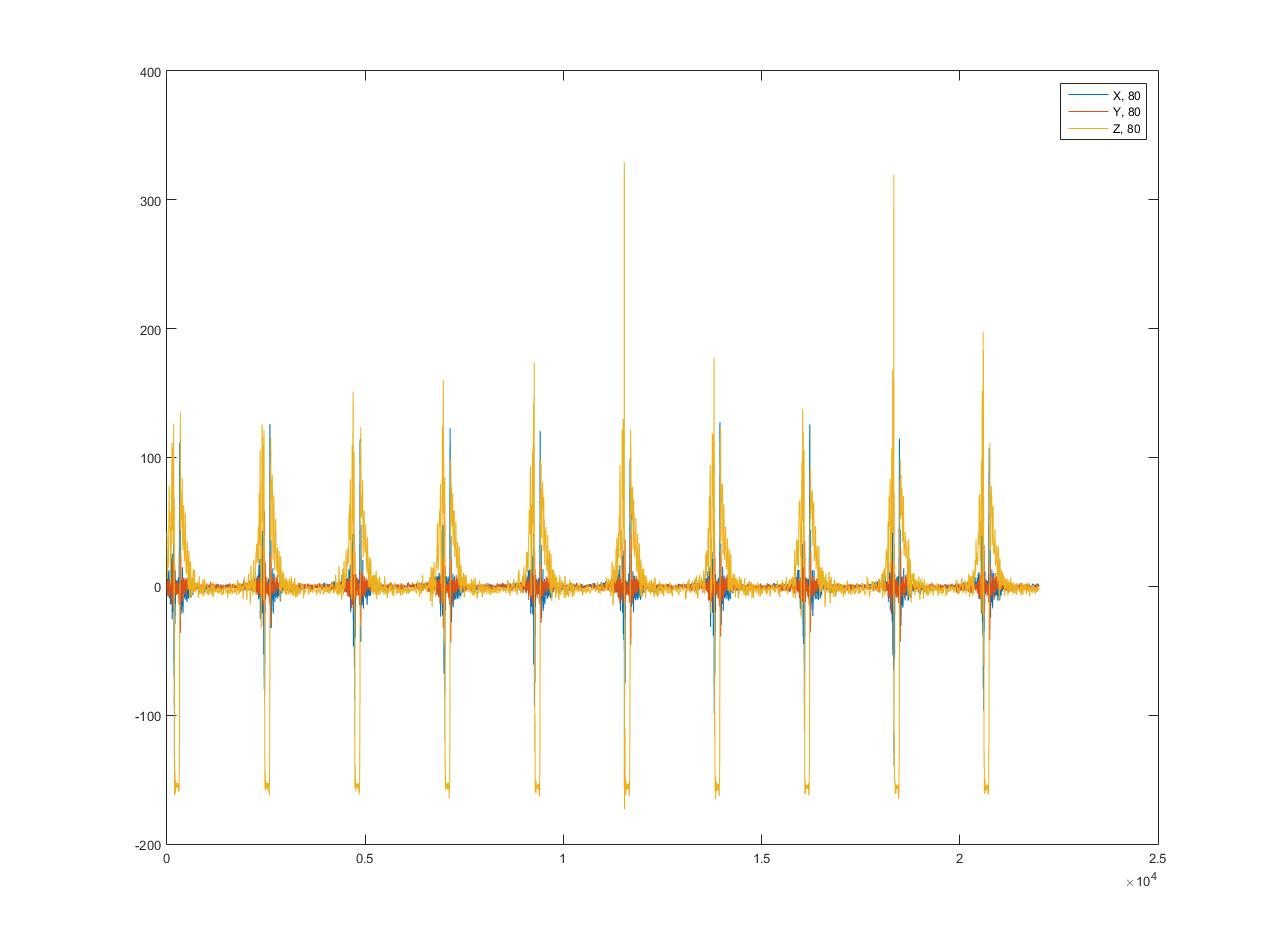
\includegraphics[height=4cm]{images/80kmh_timedomain}
\end{center}
\caption{Acceleration of inner lining of tyre at 80 km/h in time domain.}
\label{80_TD}
\end{figure}

\begin{figure}[htb]
\begin{center}
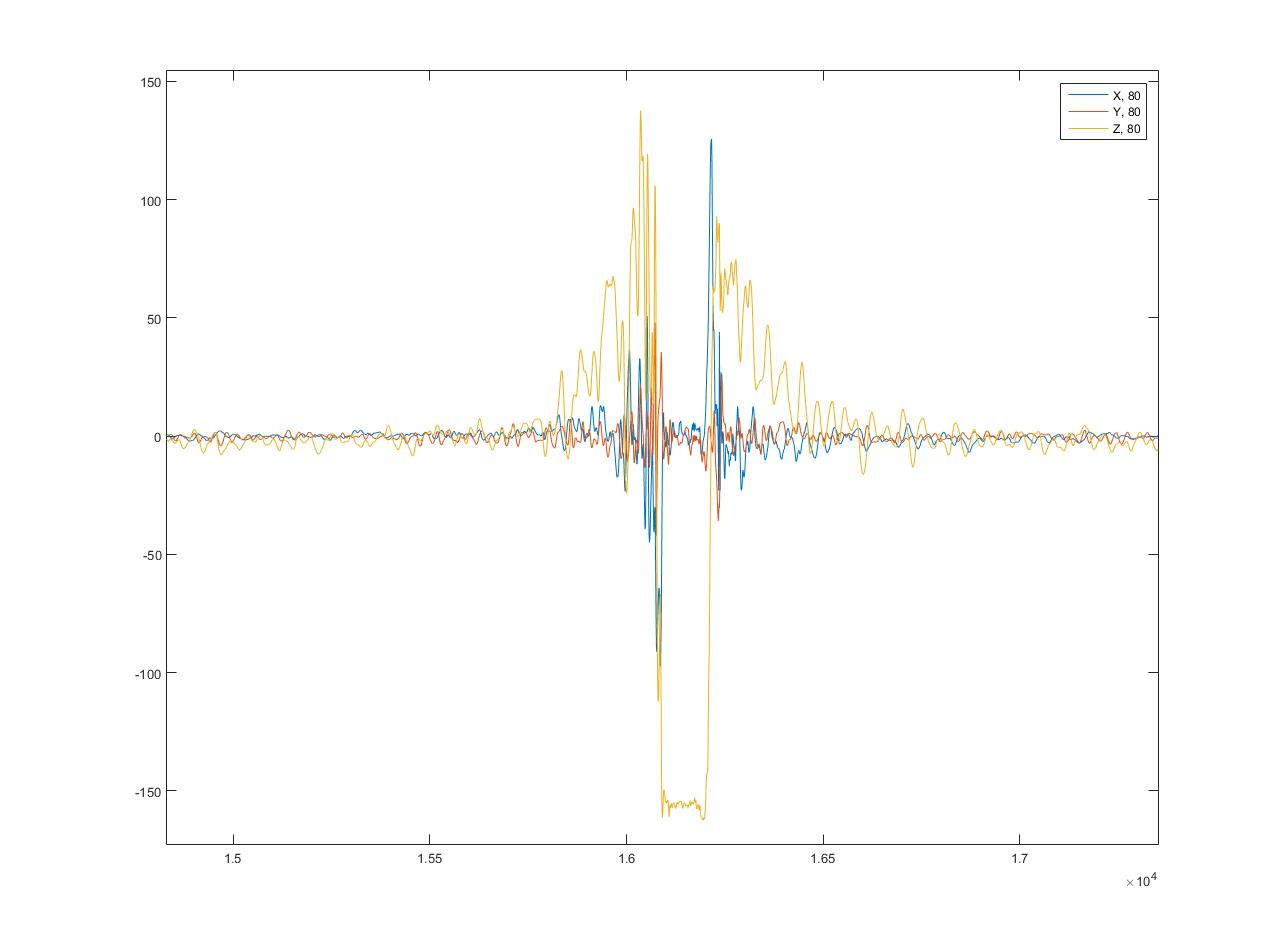
\includegraphics[height=4cm]{images/80kmh_timedomain_onerotation}
\end{center}
\caption{Acceleration of tyre inner lining in single rotation at 80 km/h. }
\label{80_TD_zoom}
\end{figure}

\begin{figure}[htb]
\begin{center}
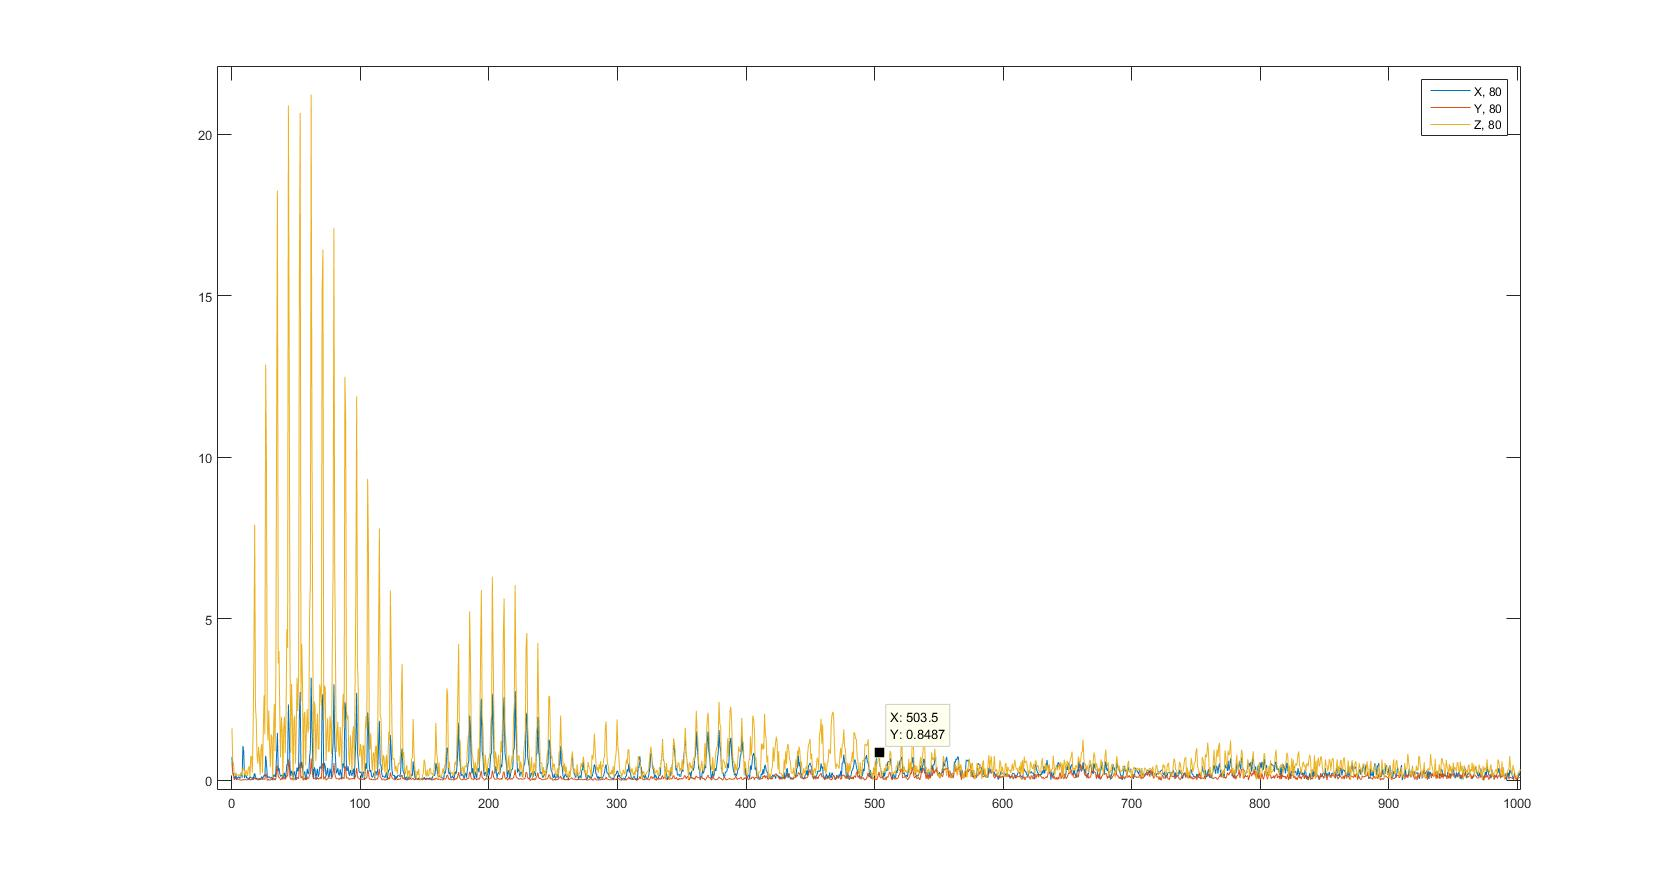
\includegraphics[height=4cm]{images/FFT-80}
\end{center}
\caption{Frequency domain representation of acceleration data.}
\label{80_FFT}
\end{figure}

\begin{figure}[htb]
\begin{center}
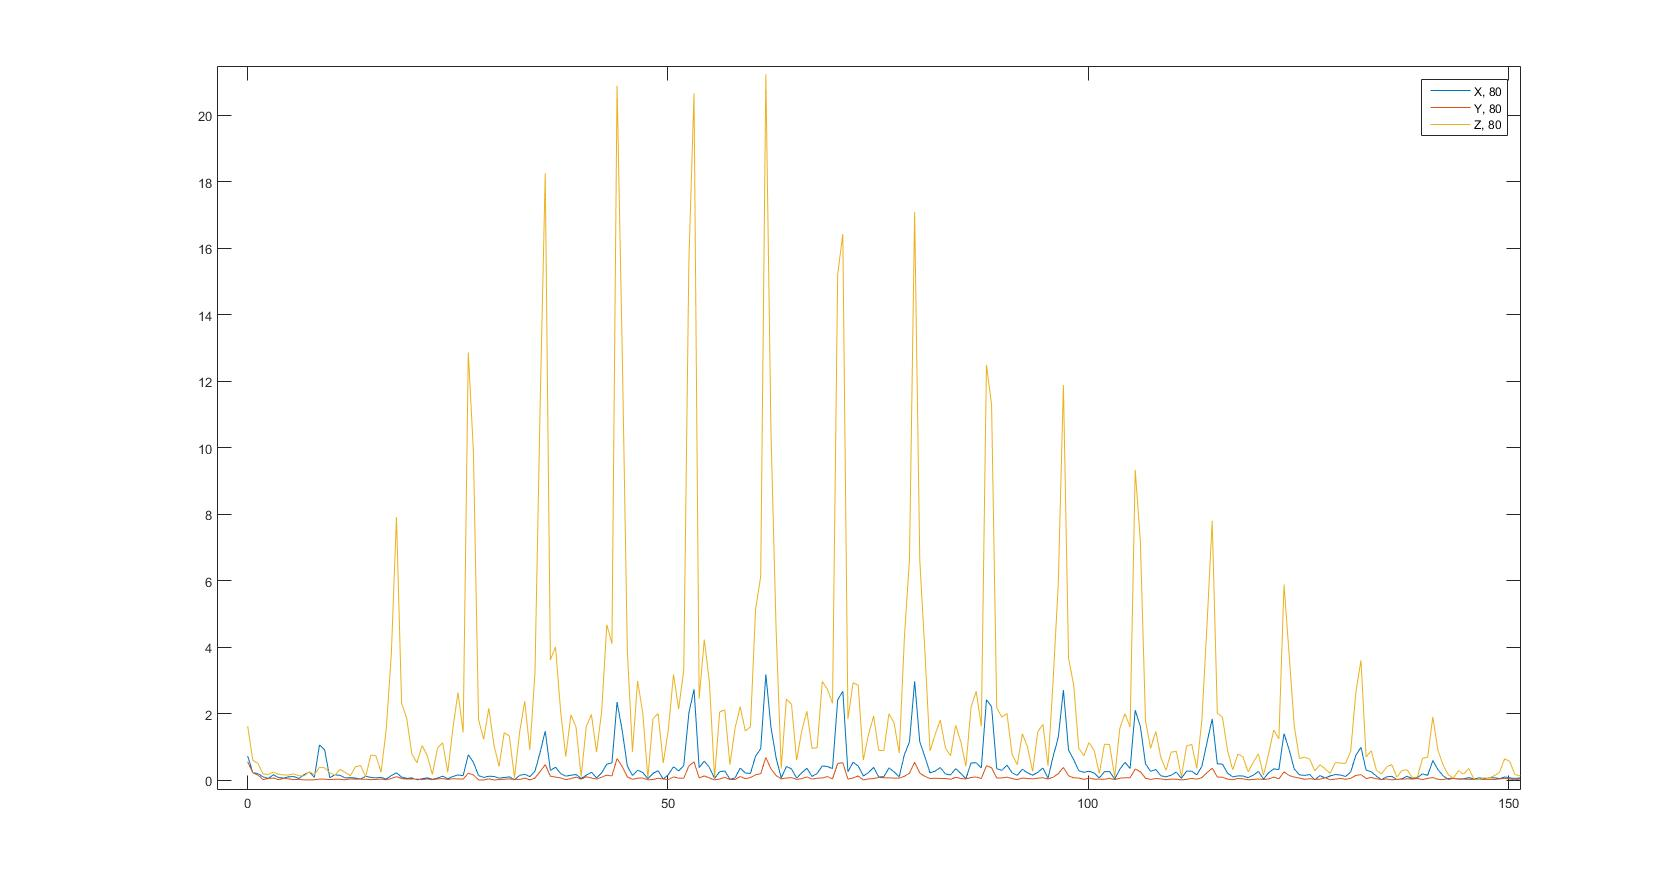
\includegraphics[height=4cm]{images/FFT-80-zoom}
\end{center}
\caption{Most of the energy is found in 10-100 Hz range.}
\label{80_FFT_zoom}
\end{figure}

It's important to notice that the sensor used was piezoelectric, which forms a highpass filter as the operation is based on charge between layers. This charge dissipates over time, so the steady-state centripetal acceleration reads as zero. There is a constant acceleration on the device caused by rotational movement by the tire. 

\subsection{Energy harvesting}
\subsubsection{Overview of methods}
First step of designing a system for energy harvesting was to identify the currently known methods and their properties. Kubba et al. \cite{Kubba2014} have done a study on tyre pressure sensor technology, they present electromagnetic, electrostatic, piezoelectric and thermal solutions as possible candidates for energy harvesting. In addition, triboelectric and magnetostrictive methods have been proposed by Bowen et al \cite{Bowen2014}. Outside of the context of tyres, Paradiso et al. \cite{Paradiso2005} present solar and radiowave harvesting techniques. Radioactive power source has been suggested by Lal et al \cite{Lal2004}. 

Electromagnetic power sources are based on Faraday's law of electromagnetic induction. A magnet and a coil are put in motion relative to each other, and the changing magnetic flux through the coils of the generator produces voltage. Current through such device is determined by load resistance. Technology is widely used in power generation, where a primary power source such as wind or flow of water provides rotation for the generator. While conventional designs use rotational movement, linear generator designs exist. Boldea and Nasar \cite{Boldea1999} provide an overview of linear generator and actuator theory. 

Electrostatic devices charge plates of a capacitor and use mechanical vibration to vary the structure of the capacitor. As the capacitance value changes with the structure, energy can be harvested from increased potential energy in capacitor. Drawback of this method is the required control electronics and high polarization voltages needed for maximal efficiency. There are also electrostatic methods which use electrets. These electrects hold constant charge and polarization for years and they can be used in electrostatic harvesters which do not require an external exitation source \cite{Boisseau2012}. As electret elements and electrostatic generators are not readily available, they have been excluded from this study.

Piezoelectric materials generate charge in response of mechanical stress. This stress can be caused by firmly attaching the piezoelectric element to a surface which deforms (simply supported) or by leaving one end of the element free-hanging while other end is fixed (cantilevered). Dynamics of the generator are very different for the different configurations, Kim et al. \cite{Kim2014a} provides a model for impact-based piezoelectric harvester while Erturk et al. have done in-depth analysis of cantilevered piezoelectric modeling \cite{Erturk2009}. 

Thermal solutions can be further diveded into subcategories. Seeback-effect where a temperature gradient in a semiconductor material causes voltage between poles of the material is widely used in temperature sensing, but to generate appreciable amounts of power large temperature gradients of over hundred \degree C are required \cite{Amatya2010} which is not practical inside tyre. Pyroelectric materials do not require differential of temperature, they generate energy when the temperature of the entire element changes \cite{Zhang2011}. As the temperature inside tyre remains rather constant over long periods of time, these methods are not practical for this application.

Triboelectricity generates power using friction between two materials, a classic example of this is Benjamin Franklin's experiments on charging various rods by rubbing them against different materials. A flexible triboelectric generator has been presented by Fan et al. \cite{Fan2012}. Triboelectric sheets are not readily available and their construction is complex, so triboelectric generation is excluded from this work. 

Magnetostrictive materials change their magnetic field in response to external mechanical sterss. This change can be utilised to create a magnetic flux through coils as in electromagnetic generators. A magnetostrictive generator was built by Wang et al. \cite{Wang2006}. 

Solar energy can be harvested by using sun as a energy source for a thermal energy harvesting or by utilizing the photovoltaic effect to generate electricity from photons hitting photovoltaic material. Photovoltaic technology is mature and widely used, but as there is no source of light inside tyre, photovoltaic methods are not suited for the application.

Radio wave harvesting uses antennas to collect energy from ambient radio transmissions, such as WiFi- and cellural signals. Patel et al \cite{Patel2014} have built a demonstration device which uses TV broadcasts as an energy source. The tyre material dampens any RF broadcasts, which makes RF energy harvesting poorly suited for the application.

Radioactive energy harvesting resembles battery or fuel cell. A radioactive material is deposited in generator near piezoelectric cantilever. Radioactive decay charges proof mass of piezoelectric cantilever until the proof mass contacts the radioactive material by electrostatic attaraction, at which point the electrical charge is balanced and piezoelectric beam begins resonant vibration as in normal piezoelectric harvesting. Such a battery has lifetime limited only by half-life of the used material. Lal and Blanchard \cite{Lal2004} present such a battery. This kind of battery would be redundant for the application, as there already exists energy in rotation of tyre which can be used to energise the cantilever. 

In conclusion, a wide range of energy harvesting technologies have been identified. As their primary properties are known, we can narrow down the suitable technology to electromagnetic, piezoelectric and magnetostrictive. These technologies are studied further to identify optimal choice for the application.

\subsubsection{Resonance-based piezoelectric harvesting}
Piezoelectric materials produce voltage in response to mechanical stress. The effect is bidirectional, piezoelectric element can also produce mechanical strain in response to applied voltage. The material has crystalline structure with electrical dipoles in balanced state when no stress is applied. Mechanical stress unbalances these dipoles, creating element which resembles electronically a charged capacitor. 

A common approach to piezoelectric harvesting is to configure the element as a cantilever and tune the resonant frequency of the system to dominant frequency of the surrounding environment. In some applications, such as in machines running at the frequency of power grid (50 HZ or 60 HZ) this kind of frequency-tuning is relatively straightforward. TODO

\subsubsection{Impact-based piezoelectric harvesting}
As the resonant harvesting is not feasible in the environment inside tire, another method would be to use an impactor to hit a piezoelectric plate on every cycle of a tire. These impacts would provide energy once per rotation of a tire. This method has been tried before by {\color{red} Cite} and it was found to provide up to 4 mW of power in average. TODO

\subsubsection{Electromagnetical harvesting}
Electromagnetical harvesting is based on Faraday's law of induction: A loop of wire acquires electromotive force (EMF) in response to a changing magnetic field. More formally:

\begin{equation}
  \varepsilon = - \frac{d \Phi_ {B}}{d t} , 
\end{equation}

where $\varepsilon$ is the EMF, $\Phi_{B}$ is magnetic flux through loop area, and $t$ is time. For a tightly wound coil of wire, the equation can be stated as 

\begin{equation} \label{eq:emf}
  \varepsilon = -N \frac{d \Phi_{B}}{d t} , 
\end{equation}

where N is the number of turns in a coil. \cite[p.999]{universityphysics}

It's important to notice that magnetic flux through wire $ \Phi_{B} $ can change for a variety of reasons: the source of field can be in motion, strength of field can vary, the coil can be in motion, and the shape of coil can vary. In energy harvesting application in an environment with vibrations motional energy is readily available, so we focus on energy harvesting methods which either move the source of magnetic field or the coil itself.

It's obvious from equation \eqref{eq:emf} that energy available increases with the strength of magnetic source, number of turns in a coil and rate of change in the magnetic field. 

Magnetic source can be either permanent magnet or a electrically induced source as in induction motors. Induction-based generators require reactive power to start up, which means that any harvester design incorporating an induction generator would need a secondary power source to start the inductive generator. Hence the focus of this thesis will be in permanent magnet designs.

\begin{figure}[htb]
\begin{center}
\includegraphics[height=4cm]{images/cited/lgm}
\end{center}
\caption{A magnetically balanced linear generator Tornincasa et al. \cite{Tornincasa2012}}.
\label{lgm}
\end{figure}

In addition to voltage available from the generator, it's important to consider source impedance. A very simple electrical equivalent model of the generator is presented in \ref{gen_simple}, where generator is presented as a voltage source in series with lumped inductor and resistor \cite{Jirutitijaroen2012}. 

\begin{figure}[htb]
\begin{center}
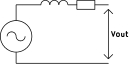
\includegraphics[height=2cm]{images/own_dwg/gen_simple}
\end{center}
\caption{A simple electromachanical generator equivalent circuit.}.
\label{gen_simple}
\end{figure}

This model is greatly simplified and it does not account for factors such as effect of electromagnetical force on mechanical structure of the generator. Even with these limitations, model is still useful as it can be used to determine an optimal load for the generator. 

The power output can be written formally as:

\begin{equation} \label{eq:gen_simple_power}
  P_{generated}(s) = \varepsilon(s)*I_{generated}(s),
\end{equation}

where $P_{generated}(s), V_{generated}(s), I_{generated}(s)$ are complex laplace-domain power, voltage and current dependent on frequency. It can be seen that power is generated only when there is a load available, as without load there is no current flow into our out of generator. Voltage is determined by EMF as described above. Current can be written as: 

\begin{equation} \label{eq:gen_simple_current}
  I_{generated}(s) = \frac{\varepsilon(s)}{Z_{generator}(s)+Z_{load}(s)},
\end{equation}

where substituting $Z_{generator}(s) $ and $ Z_{load}(s)$ are complex impedances of load and generator. This equation is valid only for linear systems, so for example rectifying and converting power with switch mode power supply (SMPS) reduces accuracy of the equation. Substituting \eqref{eq:gen_simple_current} into \eqref{eq:gen_simple_power} we obtain:

\begin{equation}
  P_{generated}(s) = \varepsilon(s)*\frac{\varepsilon(s)}{Z_{generator}(s)+Z_{load}(s)}.
\end{equation}

Total power into load can be written as:

\begin{equation} \label{eq:generator_load_power}
  P_{load}(s) = V_{generated}(s)*\frac{Z_{load}(s)}{Z_{generator}(s)+Z_{load}(s)}*\frac{V_{generated}(s)}{Z_{generator}(s)+Z_{load}(s)}.
\end{equation}

It's easy to see from \eqref{eq:generator_load_power} that if load impedance is infinite or zero, there is no power generated. It can be shown that maximum power is generated when $Z_{generator}(s) = {Z_{load}(s)}^*$. Another consideration is efficiency of the generator. The electrical efficiency is defined as ratio of power flowing into load and total power generated. It's easily seen from equation \eqref{eq:generator_load_power} that when load impedance is equal to generator impedance, efficiency is $ 50 \%$. Efficiency rises with the load impedance, which is why generators are rarely run at their maximum power. In our application the harvested power is minuscule compared to power available in tire, so it makes sense to try to match the load impedance for maximum power.

In energy harvesting application it is important to consider the validity of established theory when generator is scaled to centimetres or even smaller dimensions. Many assumptions, such as coil being tightly wound and made of thin wire might become invalid at microscale. O'Donnel et al. \cite{ODonnell2007} have done a study on the effects of scaling dimensions downwards down to millimetre range, and they concluded that power available from generator is proportional to fourth power of generator dimension for cubical generators. Another of their primary findings was that a microfabricated generator becomes more effective than a traditional wire-wound generator when design is scaled below $2 mm$ length or in $8 mm^3$ volume. It can be concluded that in this application it is reasonable to use a wire-wound generator over microfabricated one, as the generator dimensions can be an order of magnitude larger than this crossover point. 

\subsubsection{Magnetostrictive harvesting}
TODO: Magnetostrictive harvesting resembles piezoelectric harvesting. Figure \ref{magneto} shows proposed system, where magnetostrictive cantilever is sandwiched between biasing magnets and a pickup coil.  

\begin{figure}[htb]
\begin{center}
\includegraphics[height=4cm]{images/cited/magneto}
\end{center}
\caption{A magnetostrictive energy harvester by Wang et al. \cite{Wang2006}}.
\label{magneto}
\end{figure}

\begin{comment}

\subsection{Powering the sensor}
Traditionally wireless sensors have been powered with either primary or rechargeable batteries. These systems need service at regular intervals to change or recharge the batteries. In applications where battery cannot be accessed, battery lifetime often limits the lifetime of whole system. Alternative approach has been to use generators, such as fuel cells or even radioactive power sources. These systems often have a poor power density and decreasing efficiency when scaled down to small size \cite{Knight2008}. 

This work explores ways to utilise energy present in tyre to power the sensor itself. A single tyre can waste as much as 500 W of power at high speeds {\color{red} source}, so harvesting even 1/100 000ths of wasted power would be enough for a well designed low-power sensor and transmitter.

There are many different energy harvesting solutions which use fundamentally different physical principles and energy sources, such as thermal, solar, radio waves and mechanical. {\color{red} source}. As the energy harvester is inside tyre, solar harvesting is unfeasible. Radio wave harvesting methods rely on external radio transmissions for gathering power. As the device should work regardless of external environment, these methods are not suited for application. Thermal methods require significant temperature gradients {\color{red} source}, but previous work shows that car tire can reach only ambient plus few tens of \degree C {\color{red} source}. Therefore thermal methods would be ineffective. 

Mechanical energy harvesting is a natural choice, as there is abundant amount of mechanical energy available as accelerations, vibrations and centripetal force available inside the tyre. There are various different approaches for harvesting mechanical energy, including piezoelectronic, electrostatic, electromagnetic and microelectromechanical systems (MEMS) {\color{red} source}. To select optimal method for energy harvesting, more information about the characteristics of mechanical energy is required.

{\color{yellow} refer to \cite[p.10]{Kubba2014}}

The power requirements of system create additional constraints on energy harvesting method, as the energy harvester must be able to supply enough energy and power to system. In a real-world application the power management system must be able to store energy for some period of time so sensor can operate continuosly. 




As the electromagnetical harvester does not bend in any direction, it's better suited to be built straight up along Z-axis. The structure can be made strong enough to survive the shocks present without compromising on the harvester operation. A magnet can be suspended with a spring inside a coil, or by using another magnet in a repulsing configuration as presented by Torincasa et al. \cite{Tornincasa2012}. When there is vibration in addition to relatively constant centripetal force, the magnet will move along the shaft of the coil and generate electricity. Figure \ref{lgm} shows the structure of built generator. 

A non-linear spring can be utilised to keep the magnet as well centered as possible over a wide range of tyre speeds. Theoretically this non-linearity could also be used to shift the resonant frequency of generator to track the frequency of vibration inside the tyre. In practise the movement of magnet would drive the spring outside of the resonant area. 
\end{comment}
